% Created 2016-08-17 Wed 14:38
\documentclass[tikz,convert]{standalone}
\usepackage[utf8]{inputenc}
\usepackage[T1]{fontenc}
\usepackage{tikz}
\usetikzlibrary{calc,positioning,fit}

 
\author{Holger Karl}
\date{\today}
\title{}
\begin{document}
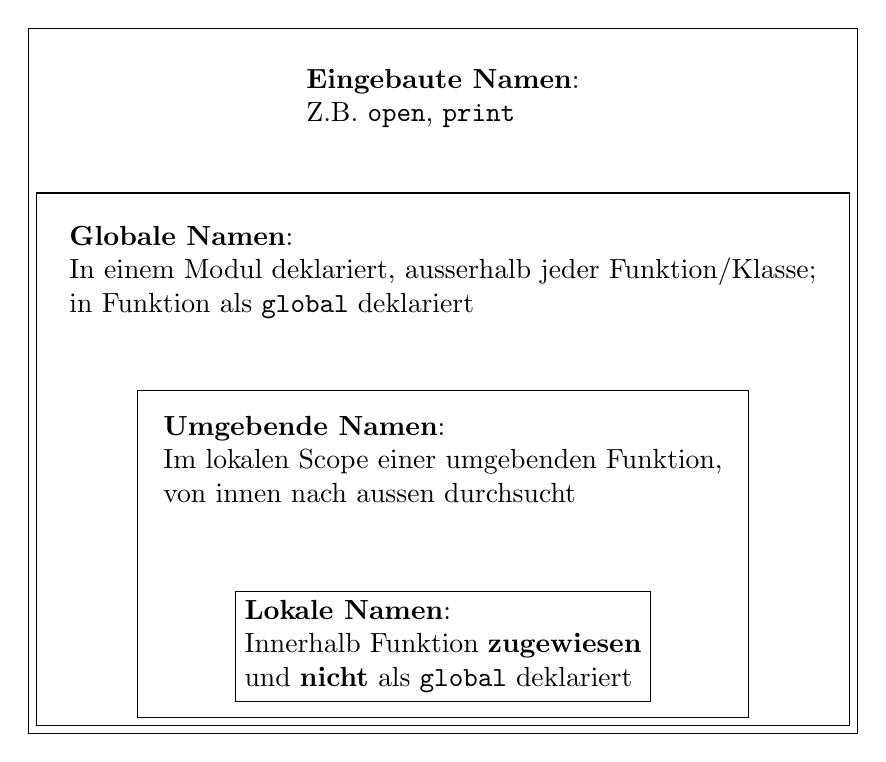
\begin{tikzpicture}

\node (builtin) [align=left] {\textbf{Eingebaute
    Namen}:\\Z.B. \texttt{open}, \texttt{print}}; 
\node (global) [below=of builtin.south,align=left] {\textbf{Globale
    Namen}:\\
  In einem Modul deklariert, ausserhalb jeder Funktion/Klasse; 
  \\in
  Funktion als \texttt{global} deklariert 
}; 
\node (encl) [below=of global.south,align=left] {\textbf{Umgebende
    Namen}:\\
  Im lokalen Scope einer umgebenden Funktion, \\von innen nach aussen durchsucht
}; 
\node (loc) [rectangle,draw,below=of encl.south,align=left] {\textbf{Lokale
    Namen}:\\
  Innerhalb Funktion \textbf{zugewiesen} \\und  \textbf{nicht} als
  \texttt{global} deklariert }; 
\node [draw,inner sep=0.2cm,fit={(encl) (loc)}] {}; 
\node [draw,inner sep=0.3cm,fit={(encl) (loc) (global)}] {}; 
\node [draw,inner sep=0.4cm, fit={(encl) (loc) (global) (builtin)}] {}; 
\end{tikzpicture}

\end{document}